\documentclass[a4paper,10pt,onecolumn,oneside,openany]{jsbook}
% 参考URL http://d.hatena.ne.jp/yosshi71jp/20101210/1292005429 感謝です
% パッケージの設定,これは不要なものもあるかもしれない
\usepackage{amsmath,amssymb}
\usepackage{bm}
\usepackage{epsbox}
\usepackage[dvipdfmx]{graphicx}
\usepackage{verbatim}
\usepackage{wrapfig}
\usepackage{ascmac}
\usepackage{makeidx}
\usepackage[dvipdfmx]{graphicx}

\usepackage{listings, jlisting}
\usepackage{color}
 
\lstset{
    language=Python,%プログラミング言語によって変える。
    numbers = left,
    numberstyle = {\tiny \emph},
    numbersep = 10pt,
    breaklines = true,
    breakindent = 40pt,
    frame = tlRB,
    frameround = ffft,
    framesep = 3pt,
    rulesep = 1pt,
    rulecolor = {\color{black}},
    rulesepcolor = {\color{black}},
    flexiblecolumns = true,
    keepspaces = false,
    basicstyle = \scriptsize,
    identifierstyle = \itshape\scriptsize,
    commentstyle = \fontfamily{ptm}\selectfont\scriptsize,
    stringstyle = \scshape\scriptsize,
    tabsize = 4, 
 }

\makeindex
%%% 余白・文字数調整(左37mm, 右18mm, 上下共30mm, 文字数約40字/行, 行数約32行)
% 実際の寸法は学科の規定に従ってくださいね
\setlength{\textwidth}{155truemm}      % テキスト幅: 210-(37+18)=155mm
\setlength{\fullwidth}{\textwidth}     % ページ全体の幅
\setlength{\oddsidemargin}{37truemm}   % 左余白
\addtolength{\oddsidemargin}{-1truein} % 左位置デフォルトから-1inch
\setlength{\topmargin}{30truemm}       % 上余白
\setlength{\textheight}{237truemm}     % テキスト高さ: 297-(30+30)=237mm
\addtolength{\topmargin}{-1truein}     % 上位置デフォルトから-1inch
% 本文の行数と桁数を指定出来るように
\def\linesparpage#1{\baselineskip=\textheight
   \divide\baselineskip by #1}
\def\kcharparline#1{%
   \ifx\xkanjiskip\undefined%
   % NTT jTeX用
   \jintercharskip 0mm plus 0.2mm minus 0.2mm
   \else
   % ASCII pTex用
   \xkanjiskip 0mm plus 0.2mm minus 0.2mm
   \fi
   \settowidth{\textwidth}{あ}%
   \multiply\textwidth by #1}
%
%
\begin{document}
\linesparpage{32} % 一ページを32行に(効果ない・・・)
\kcharparline{40} % 一行を40字に
%%% タイトル設定
\begin{titlepage}
\begin{flushright}
{\large
指導教員:来住伸子 教授 \\ % 主査
%副査:□□□□ 教授              % 副査
}
\end{flushright}
\begin{center}
\vspace{150truept}
{\huge title}\\ % タイトル
\vspace{10truept}
{\Large subtitle}\\ % サブタイトル(なければコメントアウト)
\vspace{50truept}
{\huge G13908 岩科智彩}\\ % 学籍番号 著者
\vspace{10truept}
{\huge G13924 森下汐美}\\ % 学籍番号
\vspace{50truept}
{\huge 平成29年1月13日}\\ % 提出日
\end{center}
\end{titlepage}

\frontmatter
\begin{abstract} %論文要旨
近年プログラミング教育の推進に伴い、義務教育化が進んでいる。その中で米国マサチューセッツ工科大学のメディアラボが開発したScratchは無償で提供されているグラフィックプログラミング環境である。プログラミングを行う際の命令を本ツールではブロックを組み合わせて作り上げる。初心者にとっては使いやすい構造となっているため米国では利用が増えているものの、日本のユーザーは全体の1\%にも満たない。そこで実際に本ツールで公表をされているデータを利用してより教育に用いられるツールの解析を目指す。
本ツールですでに
\begin{enumerate}
  \item 各ブロックの種類が使われている全体での割合
  \item あるプロジェクトが他ユーザーの引用関係を示したツリー構造
\end{enumerate}
が公表されている。しかしこのデータでは全体図の把握が可能であるが1つのプログラムでブロックがどのように使われているか、引用していた場合引用元からどの程度変更させたかは不明である。
従って本研究では1つのプログラムで使用されているブロックを解析し結果を出すと同時に引用元との比較を行い、関係性を導き出す。
\end{abstract}

%%% 目次
\tableofcontents
%
%
\mainmatter
%
%%% 本文ここから

\part{序論} %3部構成を取る必要がない場合もあります
\chapter{はじめに}
\section{本研究の背景}

2006年に開発されたScratchというビジュアルプログラミング環境がある。本研究ではScratchのデータを用いて教育の場で役立てる方法を導き出す。Scratchとは米国マサチューセッツ工科大学のメディアラボが開発したフリーツールであり、キーボードでコードを打つのではなくパズルのようにブロックを組み合わせてプログラムの完成させる。
近年、世界ではIT化が進み、物とインターネットを繋ぐIoTが次々と増えていく中エンジニア不足が叫ばれている。しかし世界的に見るとプログラミング分野では日本は遅れている。総務省平成26年度「教育・学習分野の情報化に係る国内外の動向と先進事例」では世界各国でプログラミング教育が活発化していることが分かる(図1.1)。日本の旧学習指導要領の必修科目では、パドコンでワードやエクセルの使い方の教育しか行っていないが、イスラエルではコンピュータの使い方よりも原理やプログラミングを教える教育が行われている。
そのため文部科学省が2016年5月19日に発表をした成長戦略素案では第4次産業革命を支える人材を強化するため情報活用能力を伸ばそうと2020年度から小学校、2021年度に中学校、2022年度には高校でプログラミング教育での必修化の予定されている。それに先駆けて国内の学校では実際にプログラミングを行う授業も増えているという。品川区立京陽小学校では2014年度よりScratchが導入され各教科の中で活用されている。例えば理科の授業で実験結果をシミュレーションするプログラムの作成にScratchが用いられているようだ。
\begin{figure}[h]
  \centering
    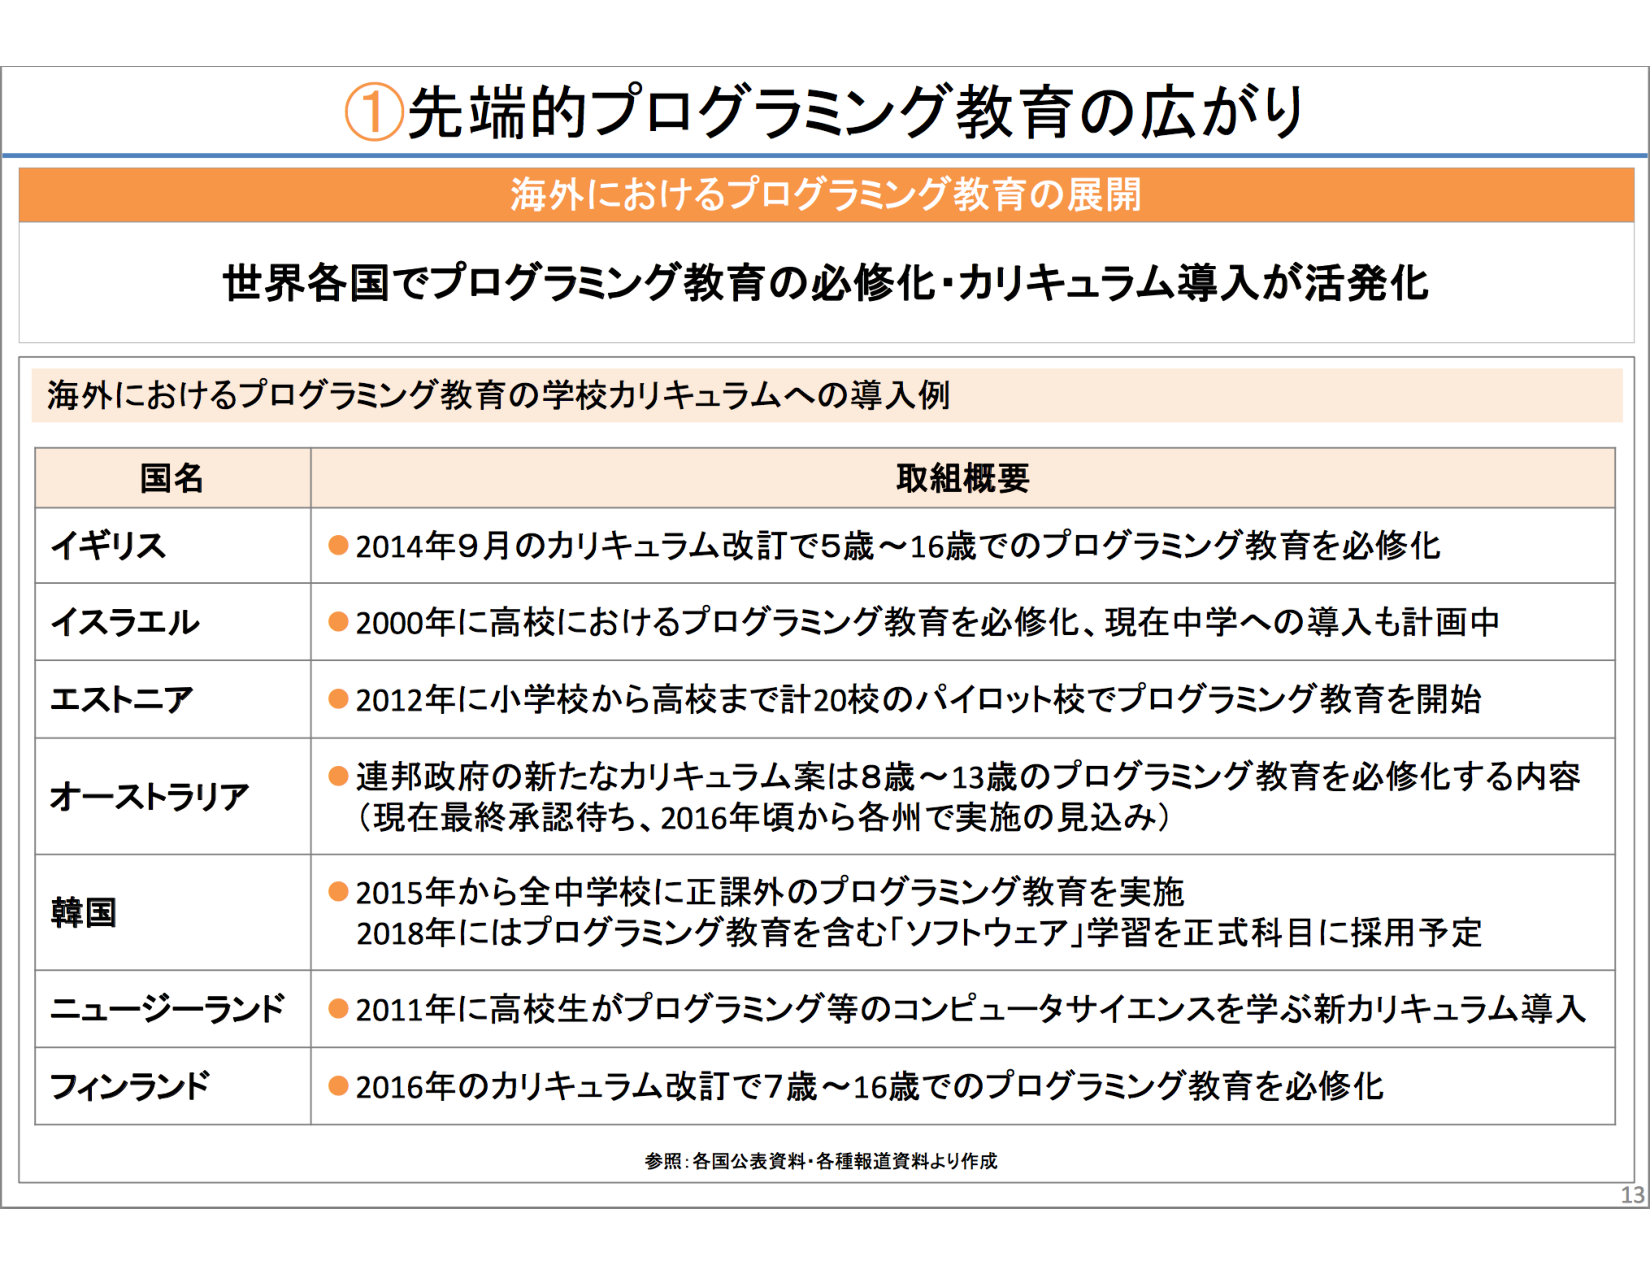
\includegraphics[scale=0.4]{graphic/foreign_data.pdf}
  \caption{平成26年度総務省 教育・学習分野の情報化に係る国内外の動向と先進事例}
 \end{figure}
 
\begin{figure}[h]
  \centering
    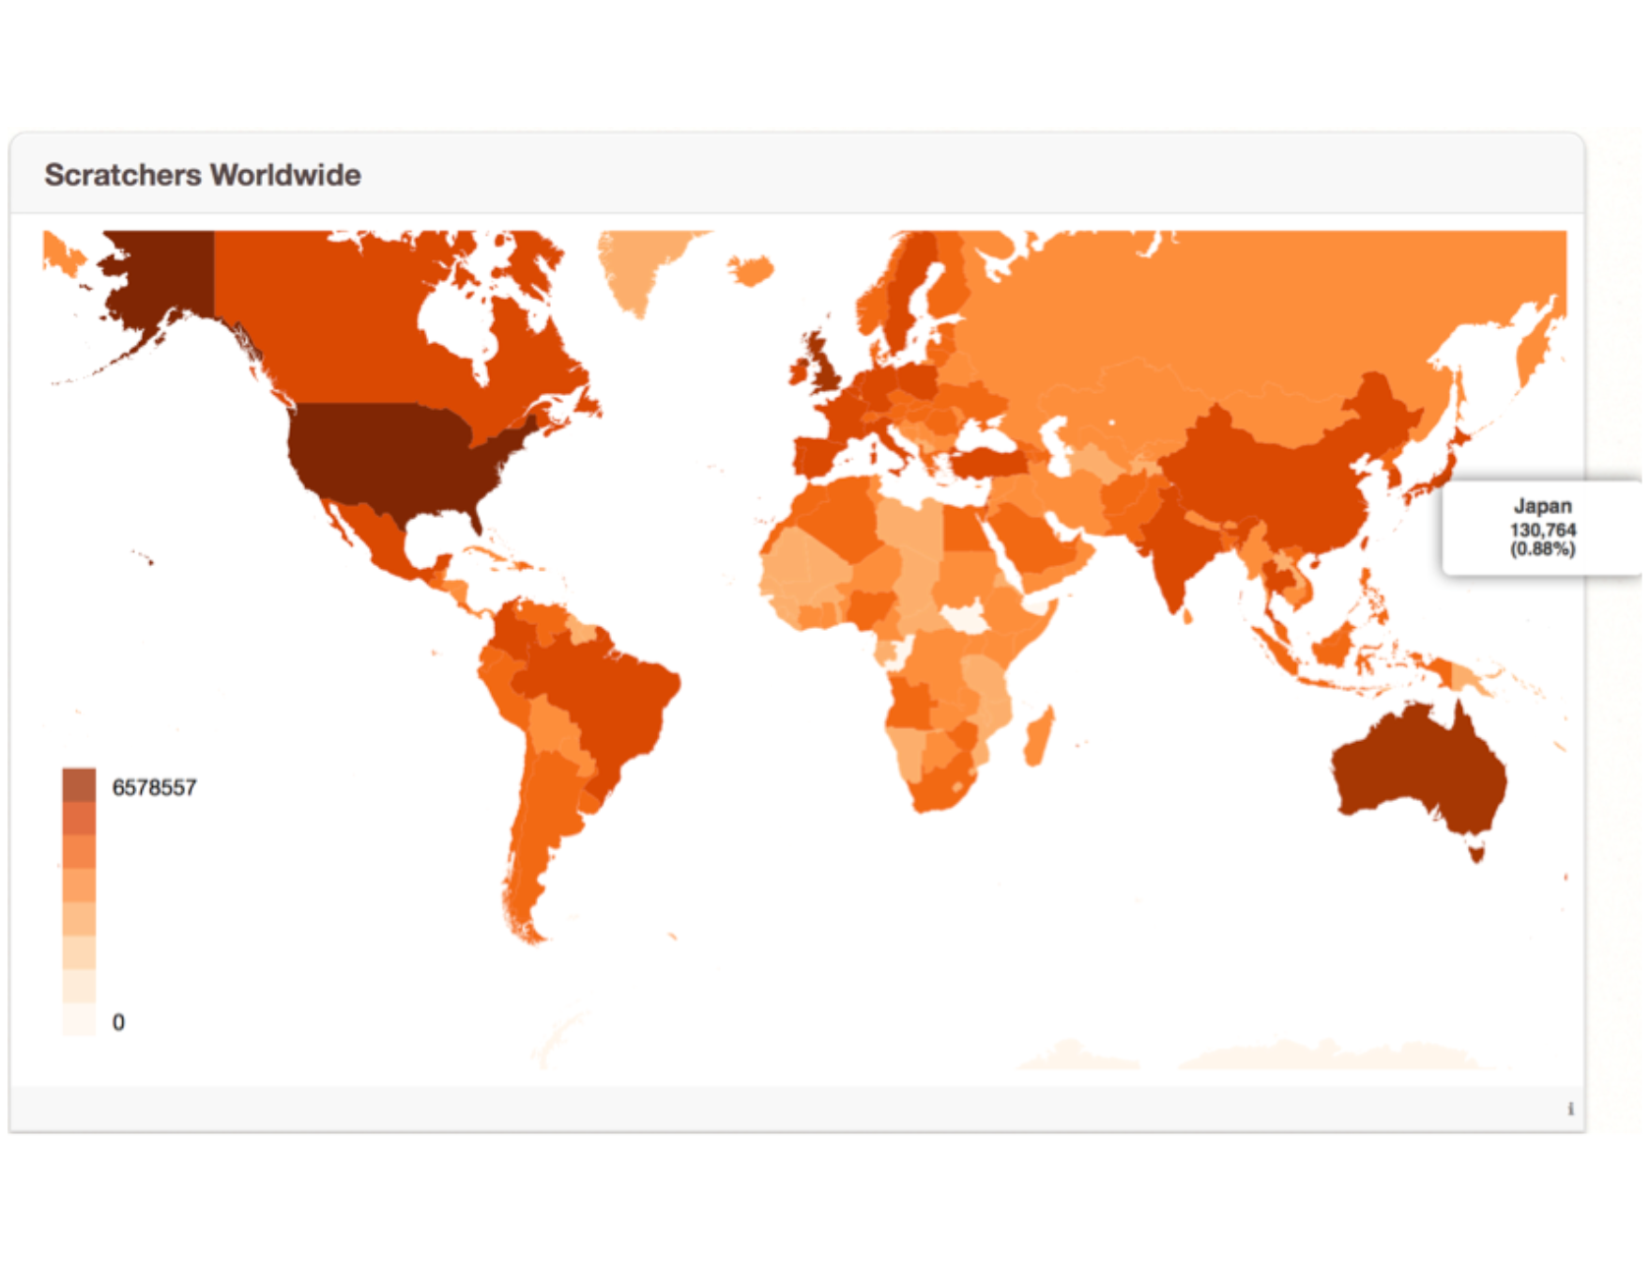
\includegraphics[scale=0.4]{graphic/world_japan.pdf}
  \caption{全世界のScratchユーザー 日本 130,764人 0.88\%}
   \end{figure}
Scratchでは全世界のユーザーのうち日本でのユーザーは現状で1%(図1.2)である。Scratch公式では利用者の数、年齢、使っているブロック等の統計データの公表があるが、Scratch自体を題材にしている先行研究は日本では数が多くない。そこで義務教育化に伴い日本でも教育現場でScratchを導入しやすくするため公開されているプログラムやデータを利用して解析を行う。

\newpage
\section{本研究の目的}

本研究ではScratchで公開されているプログラム、統計データを利用して教育現場で使いやすい新たなデータの創出を目的とする。
Scratchの現状機能を調査し、プログラミング教育における課題点を解決に導く分析を目指す。

%\section{本論文の構成}

%文章


%番号付きリスト
%\begin{enumerate}
% \item 『どんな課題を解決しようとしているのか?』%ここに項目を書く
%  \item 『その課題解決はうちの業務に役に立ちそうか?』
%  \item 仮に役に立たなくても『そのガンバリはうちの業務に役に立ちそうか?』
%\end{enumerate}


%箇条書きコード
%\begin{itemize} %ただの箇条書き,これも便利なので覚えるべし.
%  \item c++とC\#ではC\#のほうが得意です
%  \item Processingしか書けません
%  \item KinectはOpenNIもMicrosoft KinectSDKでもどっちでもいけます
%  \item 処理はGPU上で動いてます
%\end{itemize}

%クォーテーションはこう書く↓
%『なんだよさっき,``一番最初に''って言ったじゃないか!』とお怒りを受けそうだが,研究(\textit{re-search})を進める上で調査(\textit{search})をせよ,つまり先人の研究や論文検索をせよ,という前期のゼミで先生方が課しているようなアタリマエのことを述べただけであり,最初に書くのはせいぜいメモ程度,論文要旨程度の分量で構わない.

\part{本論}

%ちさちゃん
\chapter{Scratchについて}
\section{Scratchとは}
\section{Scratchの使い方}
\section{Scratchの利点、欠点}
\section{研究におけるScratchの利用意義}

%しおみ
\chapter{Scratch公式可視化データの現状}
\section{ブロックの使用頻度}

Scratch公式では無作為に選ばれたプログラムで使用されているブロックの種類を集計し、項目ごとに色を分けて使用頻度を可視化してある。高い割合の項目ほど面積が大きい。
 項目をクリックすると使用頻度の高いブロックが同じように面積が大きく表示される。この図ではScratch全体で使われているブロックの使用頻度の把握が可能である。しかしユーザー個人個人が作成したプログラムのブロックの使用頻度が分かるということではない。
 
\begin{figure}[ht]
  \centering
    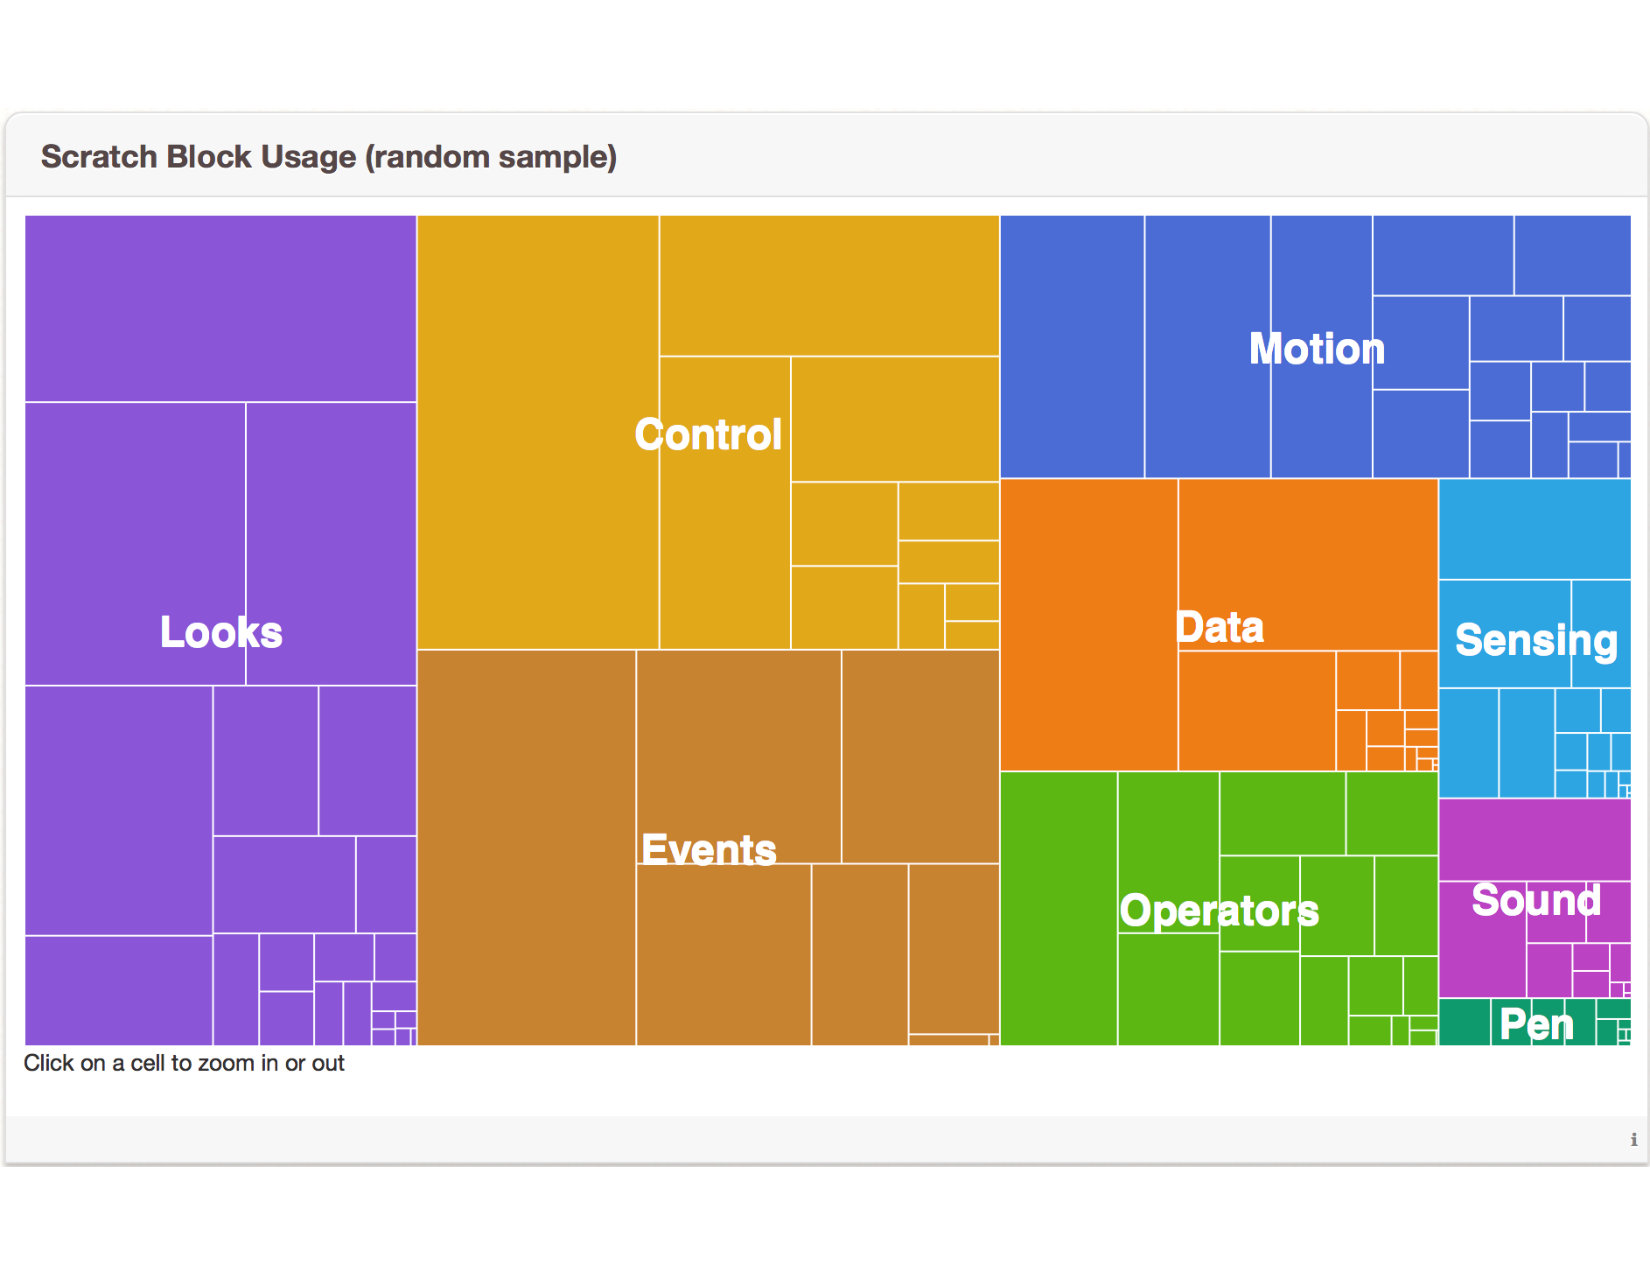
\includegraphics[scale=0.5]{graphic/scratch_block0.pdf}
  \caption{全ユーザーブロック使用度}
 \end{figure}
 
 \begin{figure}[ht]
  \centering
    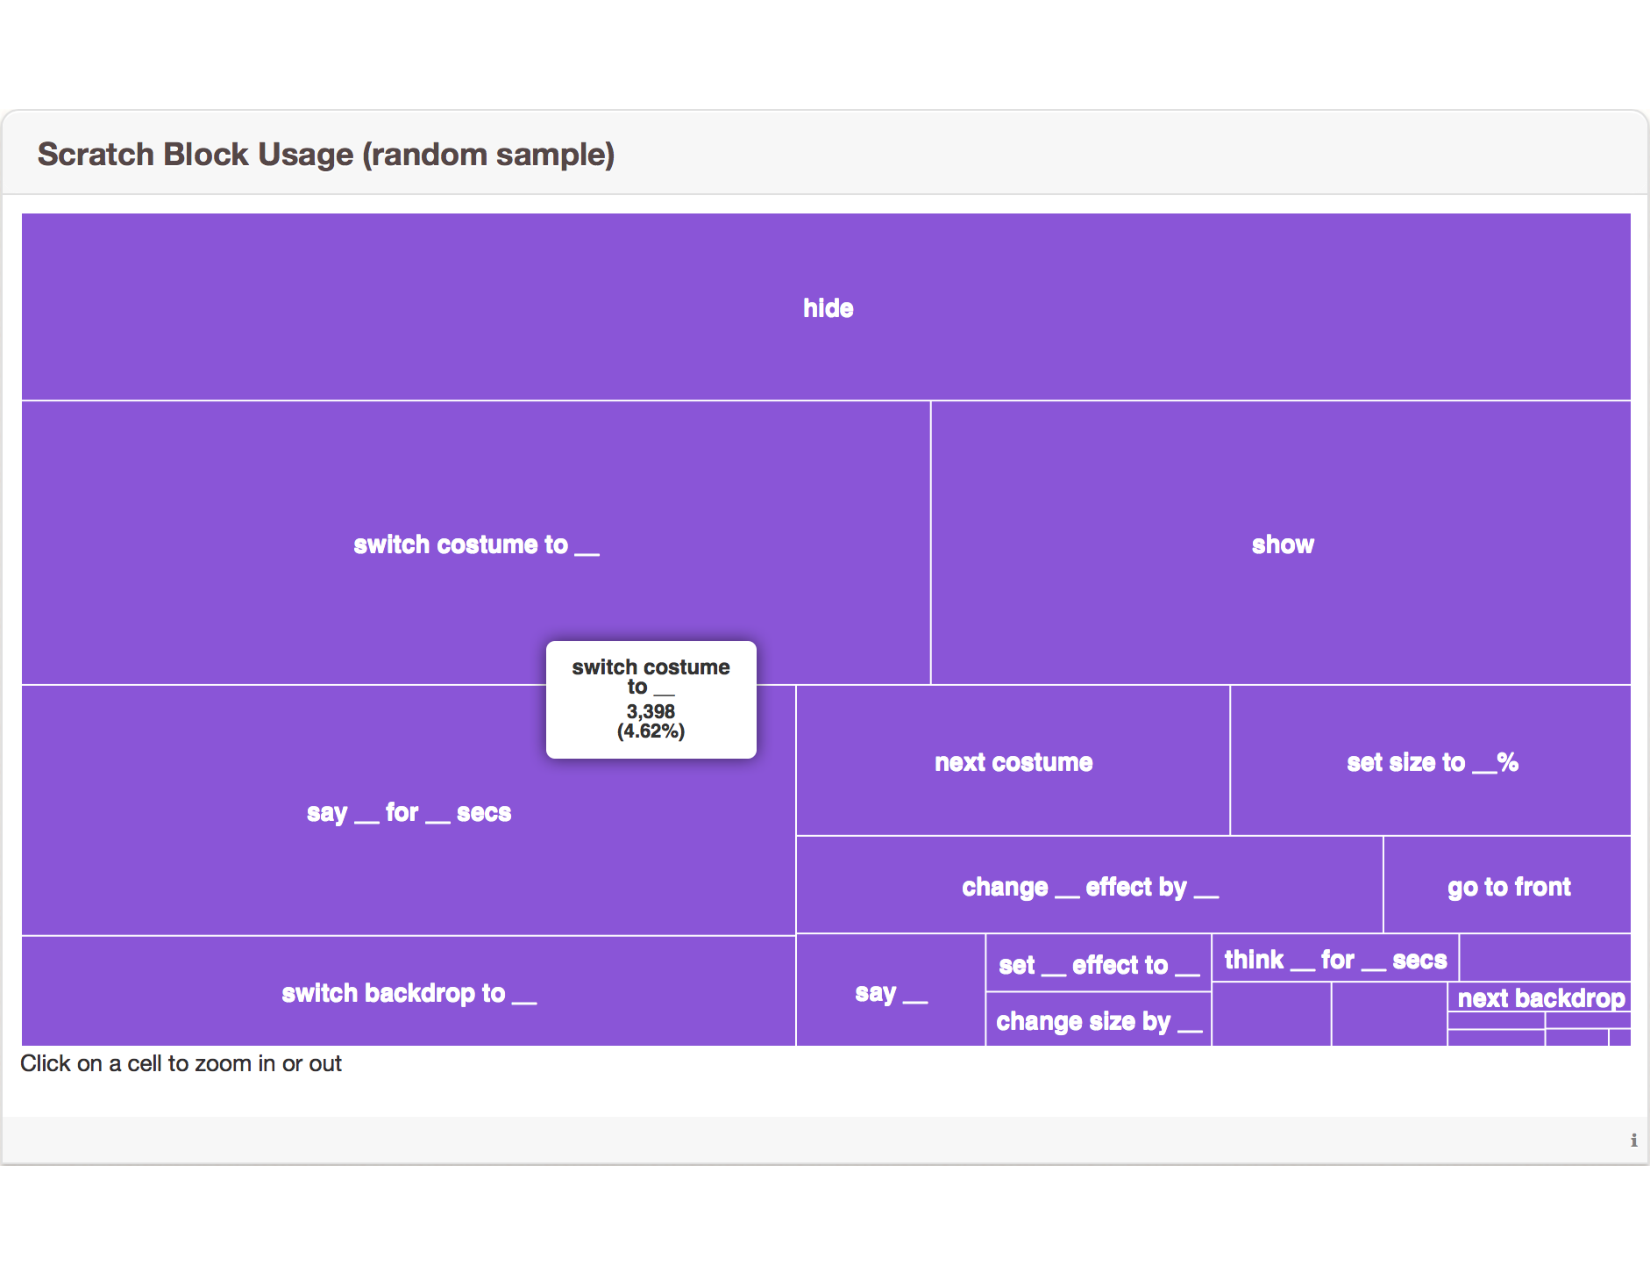
\includegraphics[scale=0.5]{graphic/scratch_block.pdf}
  \caption{全ユーザーブロック費用頻度 Locks(制御ブロック)をクリックした時}
 \end{figure}
 
 
 
\section{Remixツリー}
木構造になっているリミックスツリーは根元のプログラムを元として引用関係を表している。さらに引用されたプログラムを引用した場合も反映される。この図のデメリットはどのくらい変更が加えられているかがわからない点から元のプログラムと先端のプログラムの差を把握することは不可能である。

\begin{figure}[ht]
  \centering
    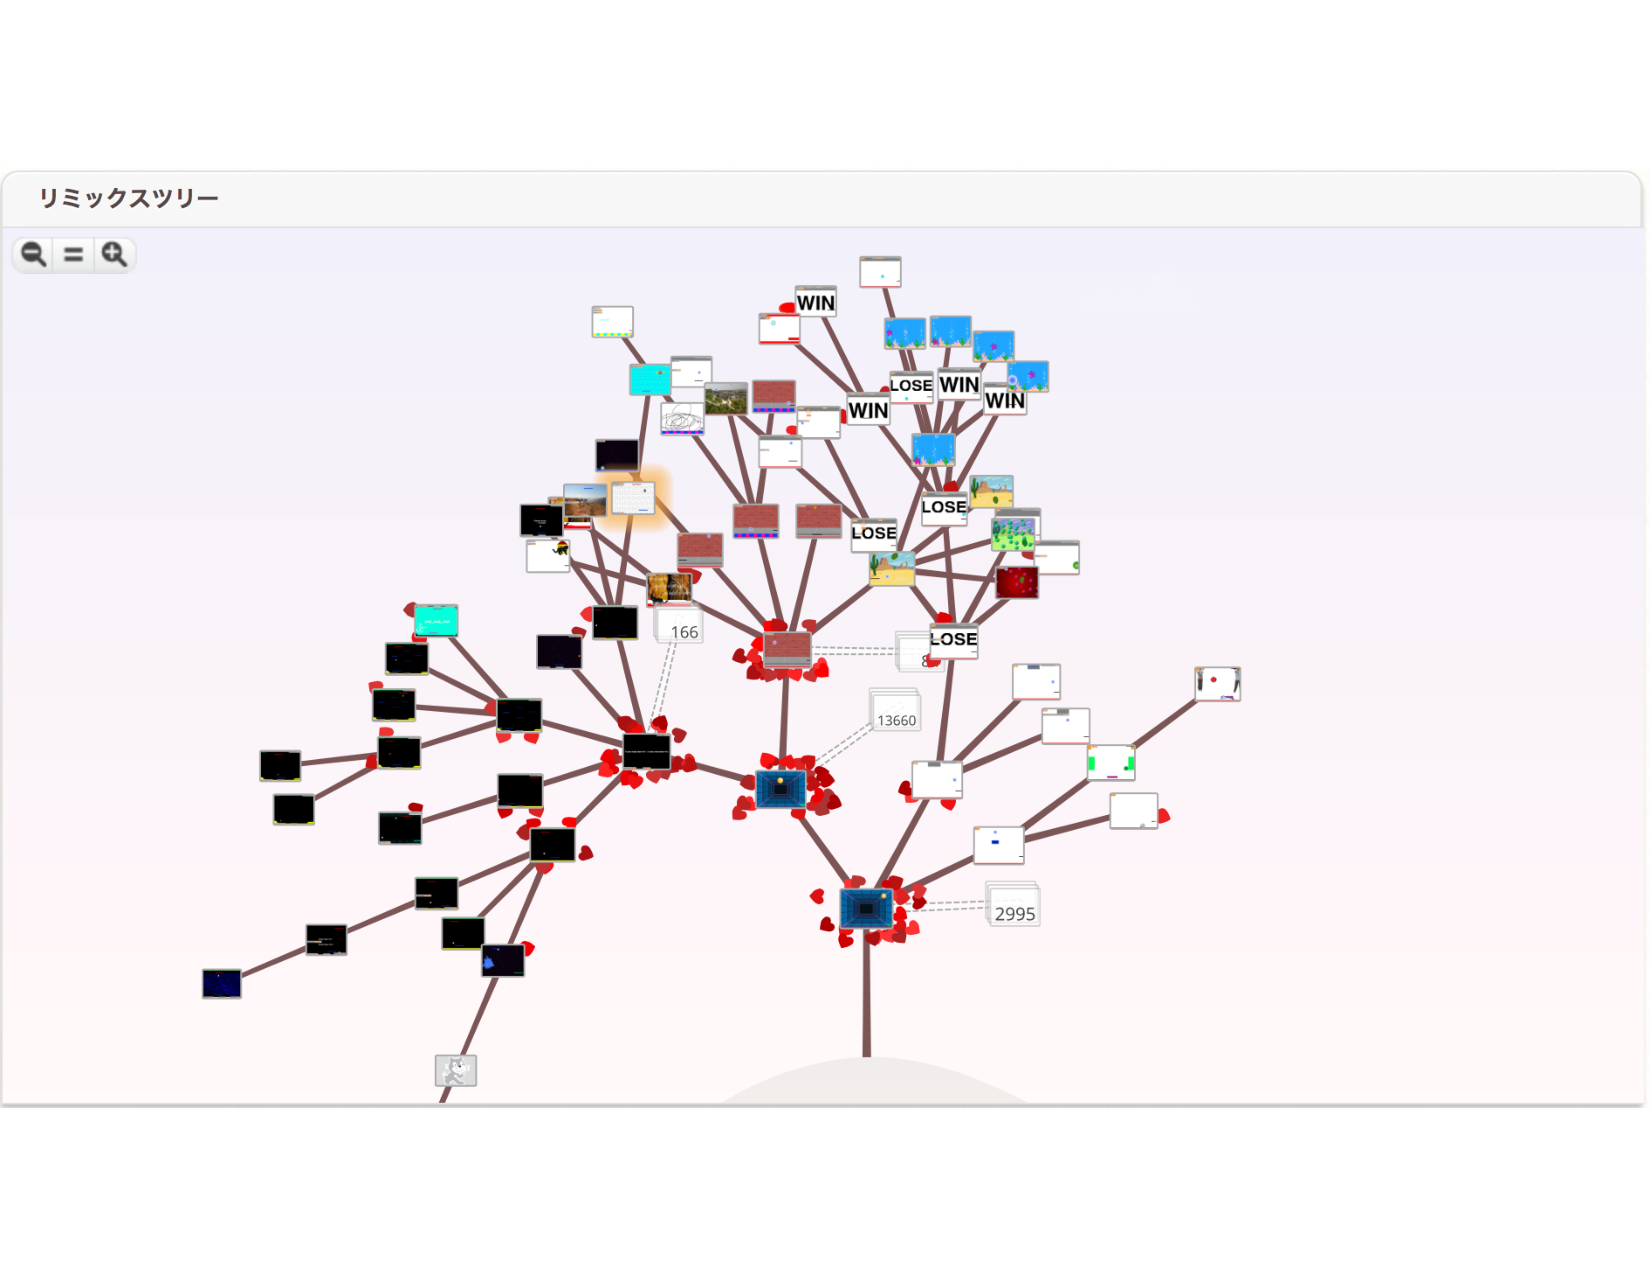
\includegraphics[scale=0.5]{graphic/remixtree_all.pdf}
  \caption{Pong Starter のリミックスツリー}
 \end{figure}

\begin{figure}[hb]
  \centering
    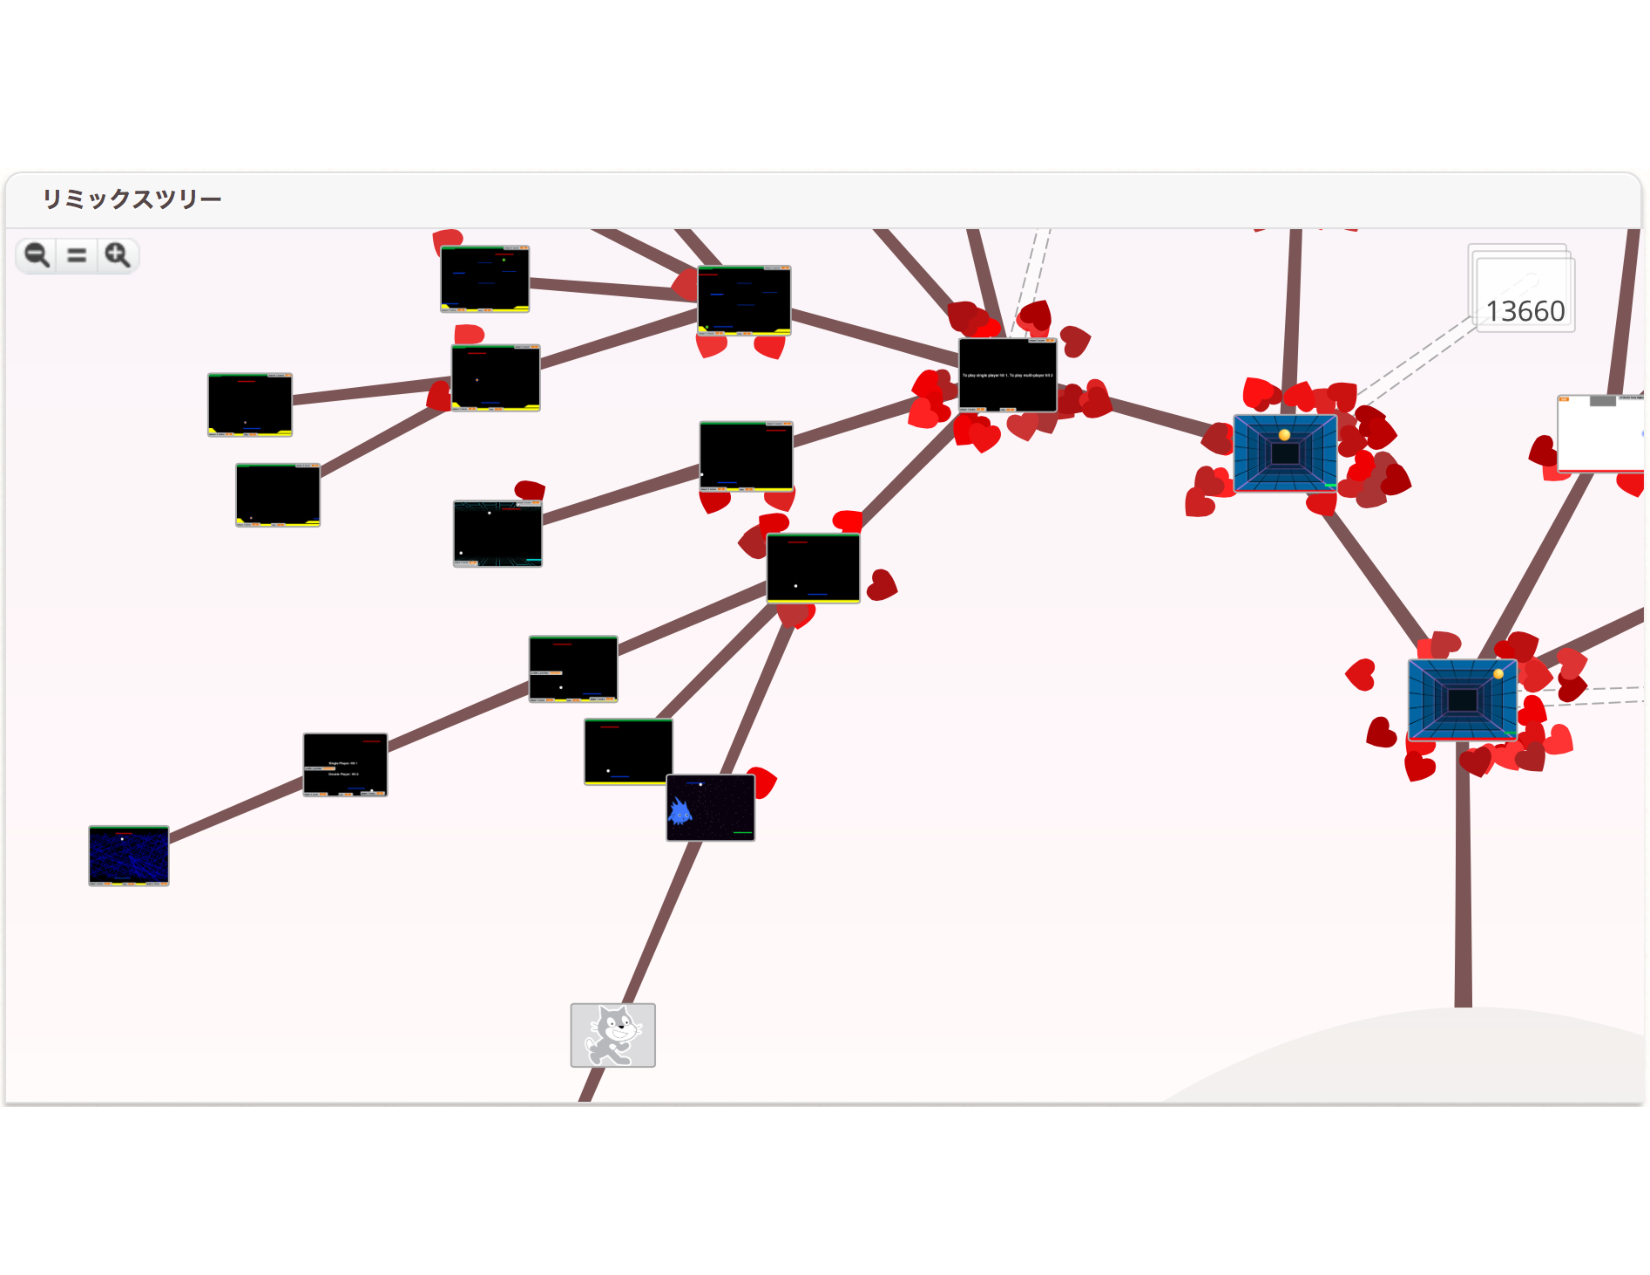
\includegraphics[scale=0.5]{graphic/remixtree_detail.pdf}
  \caption{Pong Starter のリミックスツリー 左下詳細}
 \end{figure}
 
 


\chapter{制作内容}
\section{分析内容}
%\subsection{ブロックの種類の集計}
\subsection{cos類似度の計算}
\lstinputlisting[caption=cos類似度の計算]{cosSample.py}
\subsection{ブロックとスプライトの合計数}
\lstinputlisting[caption=ブロックの合計]{countSample.py}
\lstinputlisting[caption=scratchAnalysis.py]{scratchAnalysis.py}
\lstinputlisting[caption=SimCalculator.py]{SimCalculator.py}
\section{グラフ化}

\subsection{cos類似度とブロック数のグラフ}
\begin{figure}[h]
  \centering
    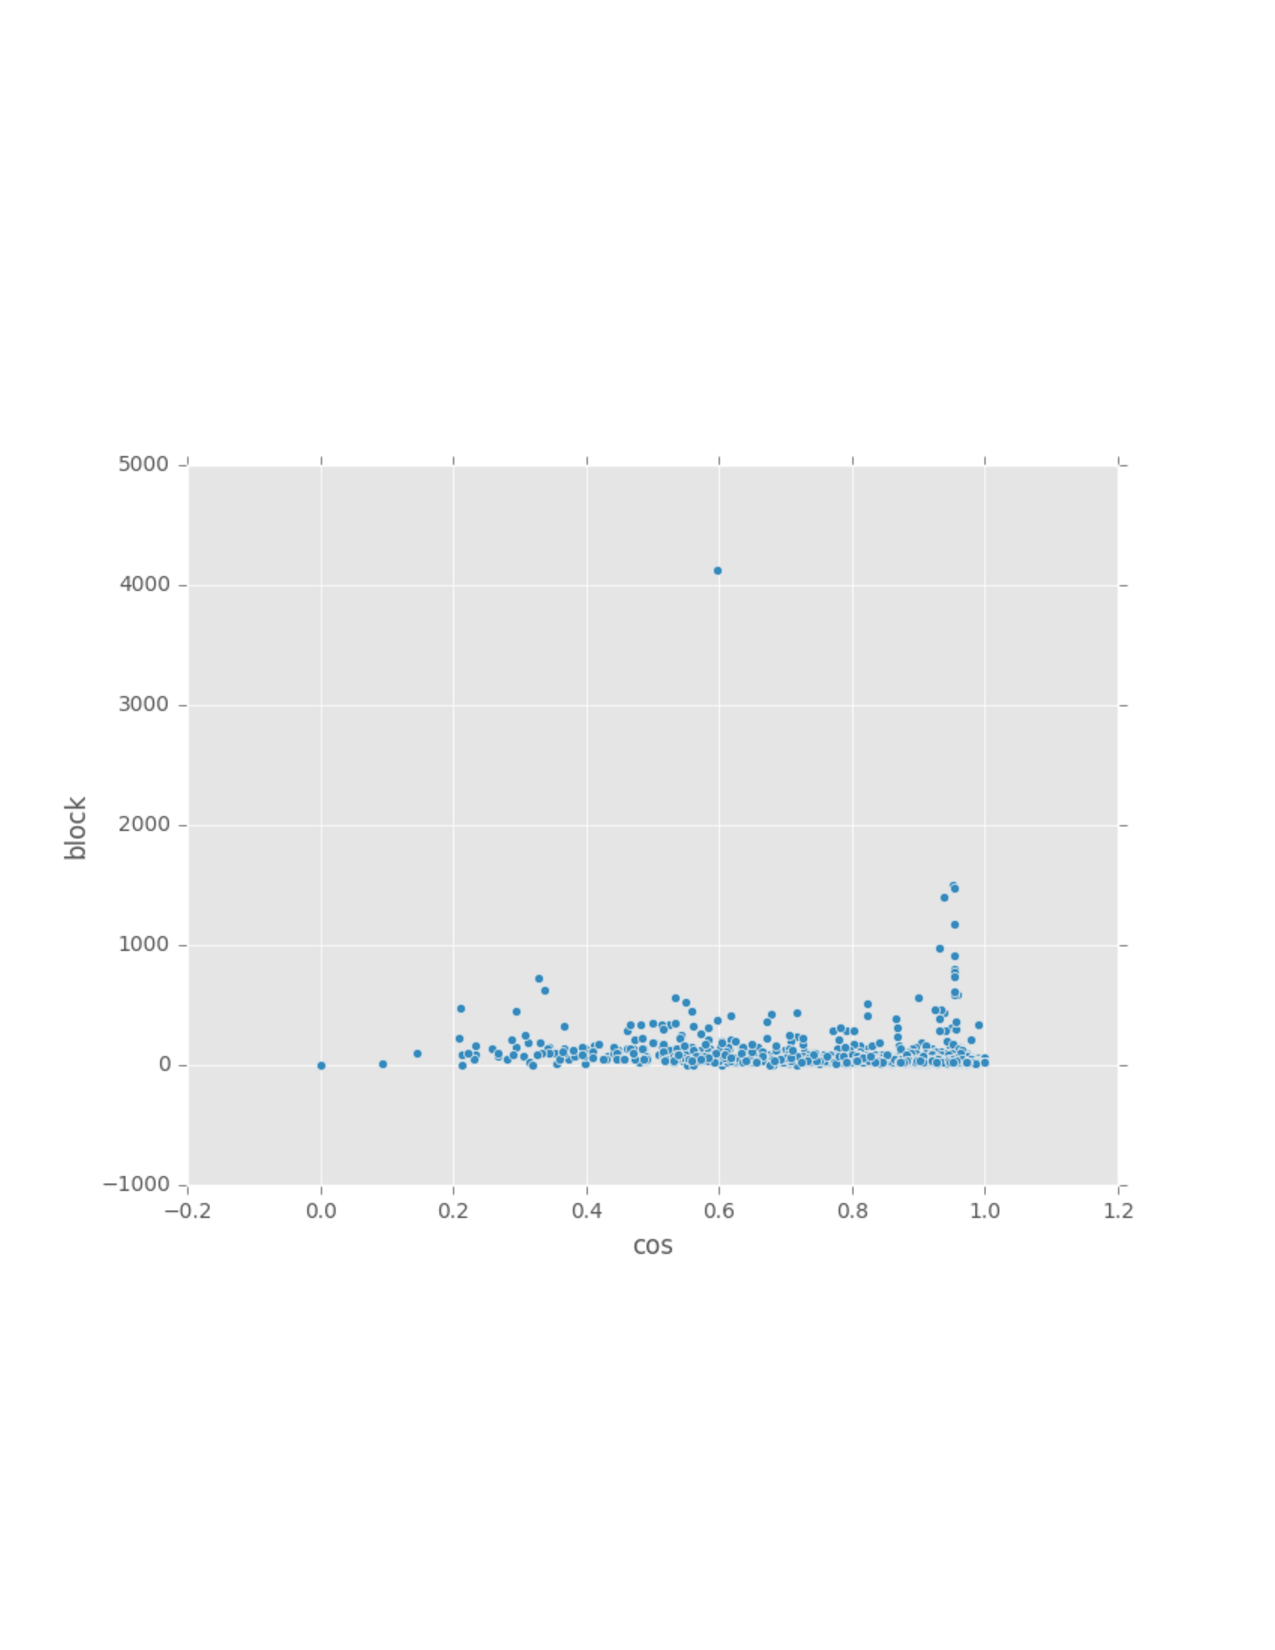
\includegraphics[scale=0.8]{graphic/block_graph.pdf}
  \caption{cos類似度とブロック数のグラフ}
 \end{figure}
 
 
\subsection{cos類似度とスプライト数のグラフ}
\begin{figure}[h]
  \centering
    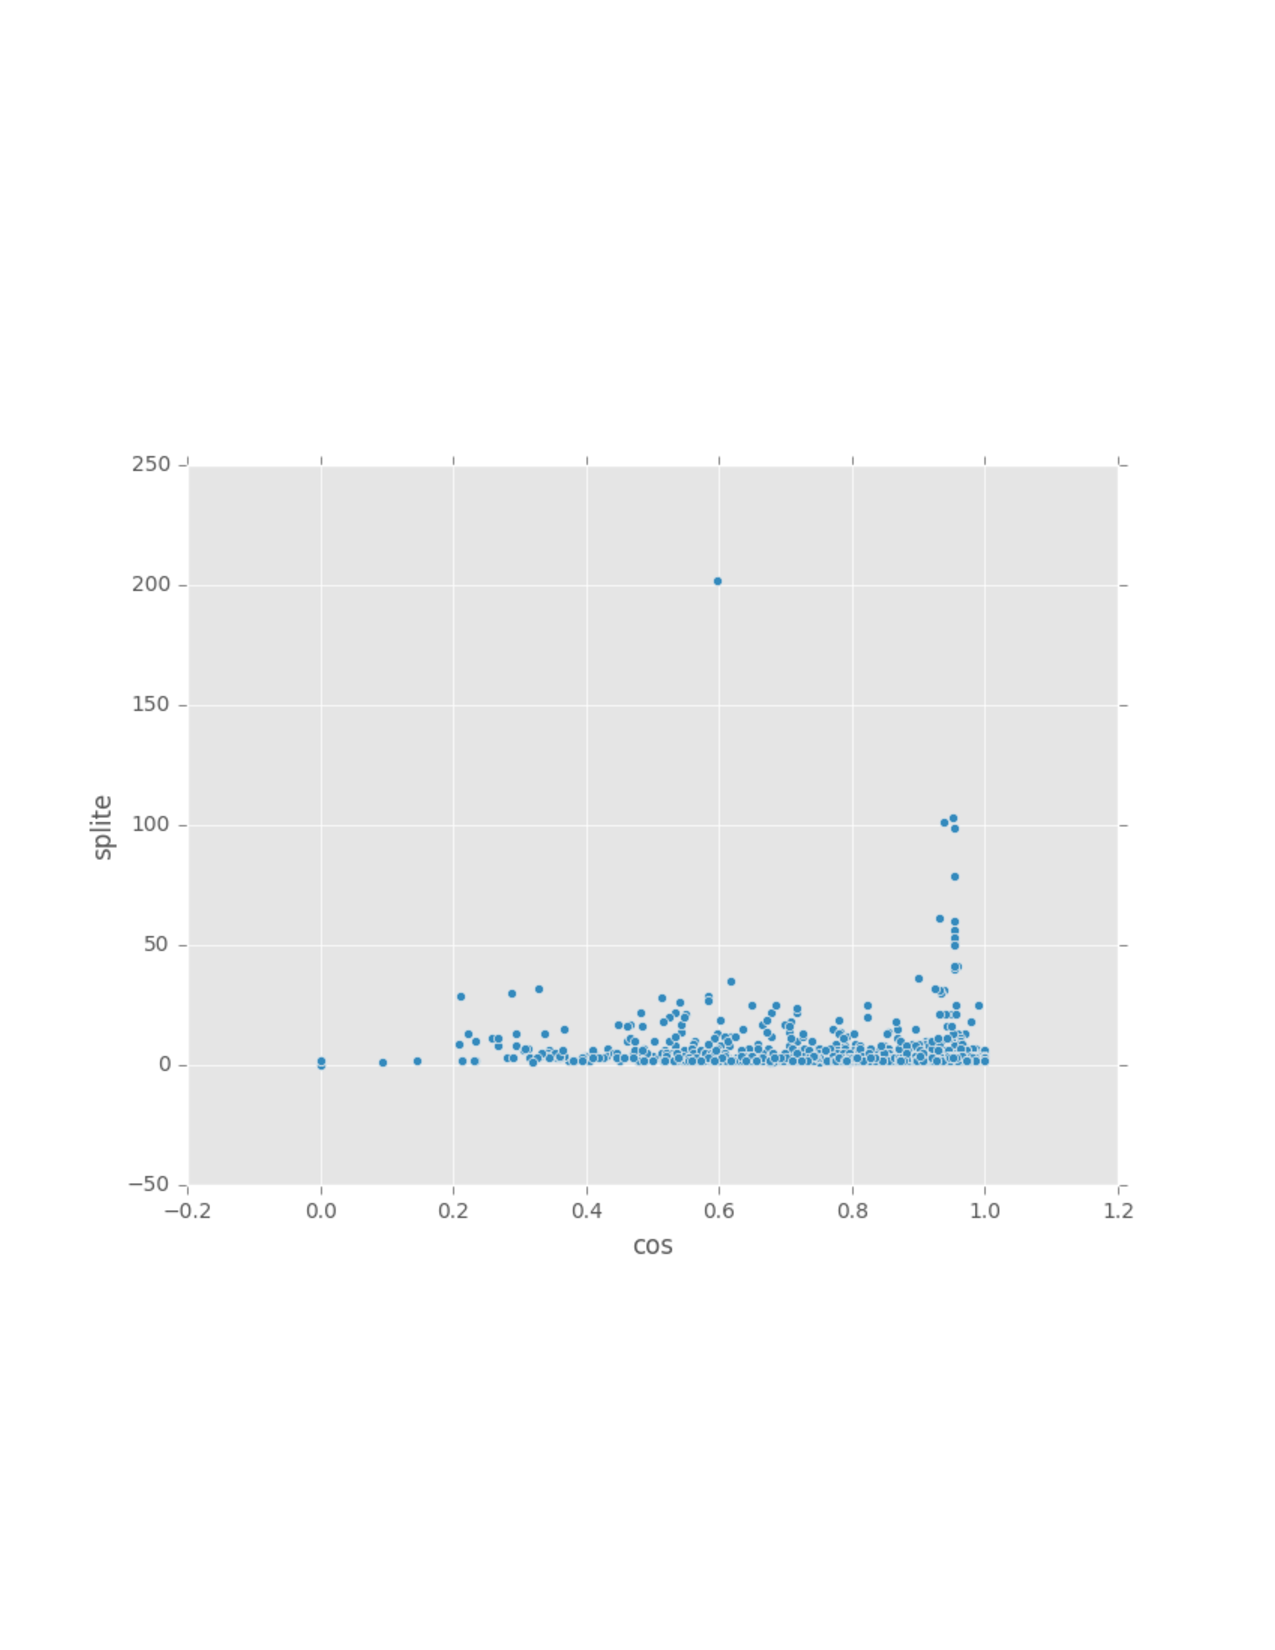
\includegraphics[scale=0.8]{graphic/spl_graph.pdf}
  \caption{cos類似度とスプライト数のグラフ}
 \end{figure}



% 図の挿入
%\begin{figure}[htbp]
%  \begin{center}
%    \includegraphics[bb=0 0 432 576,width=5cm]{figall/phd101212s.png}
%  \end{center}
%  \caption{Piled Higher and Deeper:「``FINAL''.doc」(10/12/2012)より http://www.phdcomics.com/ 参照}
%  \label{http://www.phdcomics.com/comics/archive.php?comicid=1531}
%\end{figure}

%\input{dq.txt} %新しいページから始める場合は\include, \inputの場合は改頁しない

\part{結論}
\chapter{評価}
\section{類似研究者}
\subsection{吉田葵先生}
\subsection{来住伸子先生}

\chapter{結論}


%
%%% 謝辞
\chapter{謝辞}
\addcontentsline{toc}{chapter}{謝辞}
%
%
%
\chapter{参考文献}
%\bibliographystyle{sieicej} % 電子情報通信学会の論文誌スタイルになってる
%\bibliography{myrefs}

\begin{thebibliography}{99}
%\bibitem{ohno}
%大野義夫編,\TeX\ 入門,
%共立出版,東京,1989. 

%\bibitem{Seroul}
%R. Seroul and S. Levy, A Beginner's Book of \TeX, 
%Springer-Verlag, New York, 1989. 

%\bibitem{nodera1}
%野寺隆志,楽々\LaTeX{},
%共立出版,東京,1990. 

%\bibitem{itou}
%伊藤和人,\LaTeX\ トータルガイド,
%秀和システムトレーディング,1991. 

%\bibitem{nodera2}
%野寺隆志,今度こそ\AmSLaTeX{},
%共立出版,東京,1991. 

\bibitem{tex}
D.E. クヌース,改訂新版 \TeX\ ブック,
アスキー出版局,東京,1992. 

\bibitem{jiyuu}
磯崎秀樹,\LaTeX\ 自由自在,
サイエンス社,東京,1992. 

%\bibitem{impress}
%鷺谷好輝,日本語 \LaTeX\ 定番スタイル集,
%インプレス,東京,1992--1994. 

\bibitem{Bech}
S. von Bechtolsheim, \TeX\ in Practice, 
Springer-Verlag, New York, 1993. 

%\bibitem{Gr}
%G. Gr\"{a}tzer, 
%Math into \TeX\,--\,A Simple Introduction to \AmSLaTeX, 
%Birkh\"{a}user, 1993.

\bibitem{hujita}
藤田眞作,
化学者・生化学者のための\LaTeX---パソコンによる論文作成の手引,
東京化学同人,東京,1993. 

%\bibitem{styleuse}
%古川徹生,岩熊哲夫,
%\LaTeX\ のマクロやスタイルファイルの利用(styleuse.tex),1994. 

\bibitem{Ase}
阿瀬はる美,てくてく\TeX{},
アスキー出版局,東京,1994. 

\bibitem{Walsh}
N. Walsh, Making \TeX\ Work, 
O'Reilly \& Associates, Sebastopol, 1994. 

\bibitem{Salomon}
D. Salomon, The Advanced \TeX\ book, 
Springer-Verlag, New York, 1995.

\bibitem{hujita2}
藤田眞作,\LaTeX\ マクロの八衢,
アジソン・ウェスレイ・パブリッシャーズ・ジャパン,東京,1995. 

\bibitem{Nakano}
中野賢,日本語 \LaTeXe\ ブック,
アスキー出版局,東京,1996. 

\bibitem{Fujita4}
藤田眞作,\LaTeXe\ 階梯,
アジソン・ウェスレイ・パブリッシャーズ・ジャパン,東京,1996. 

\bibitem{otobe}
乙部巌己,江口庄英,
p\LaTeXe\ for Windows\ Another Manual,
ソフトバンク パブリッシング,東京,1996--1997. 

\bibitem{Abrahams}
% P.W. Abrahams, \TeX\ for the Impatient,
% (Addison-Wesley, 1992). 
ポール W. エイブラハム,明快 \TeX{},
アジソン・ウェスレイ・パブリッシャーズ・ジャパン,東京,1997. 

\bibitem{Eguchi}
江口庄英,Ghostscript Another Manual,
ソフトバンク パブリッシング,東京,1997. 

\bibitem{FMi1}
% M. Goossens, F. Mittelbach, and A. Samarin, The \LaTeX\ Companion, 
% Addison-Wesley, Reading, 1994. 
マイケル・グーセンス,フランク・ミッテルバッハ,アレキサンダー・サマリン,
\LaTeX\ コンパニオン,アスキー出版局,東京,1998. 

\bibitem{Eijkhout}
% V. Eijkhout, \TeX\ by Topic, Addison-Wesley, Wokingham, 1991. 
ビクター・エイコー,\TeX\ by Topic---\TeX\ をよく深く知るための39章,
アスキー出版局,東京,1999. 

\bibitem{latex}
%レスリー ランポート,文書処理システム\LaTeX{},
%アスキー出版局,東京,1990. 
レスリー・ランポート,文書処理システム \LaTeXe{},
ピアソンエデュケーション,東京,1999. 

\bibitem{Okumura3}
奥村晴彦,[改訂版]\LaTeXe\ 美文書作成入門,
技術評論社,東京,2000. 

\bibitem{FMi2}
% M. Goossens, S. Rahts, and  F. Mittelbach,  
% The \LaTeX\ Graphics Companion (Addison-Wesley, 1997).
マイケル・グーセンス,セバスチャン・ラッツ,フランク・ミッテルバッハ,
\LaTeX\ グラフィックスコンパニオン,アスキー出版局,東京,2000. 

\bibitem{FGo1}
% M. Goossens, and S. Rahts, 
% The \LaTeX\ Web Companion, Addison-Wesley,  1999.
マイケル・グーセンス,セバスチャン・ラッツ,
\LaTeX\ Web コンパニオン---\TeX\ とHTML/XML の統合,
アスキー出版局,東京,2001. 

\bibitem{PEn}
ページ・エンタープライゼス\<(株)\<,
\LaTeXe\ マクロ \& クラスプログラミング基礎解説,
技術評論社,東京,2002. 

\bibitem{Fujita5}
藤田眞作,\LaTeXe\ コマンドブック,
ソフトバンク パブリッシング,東京,2003. 

\bibitem{Yoshinaga}
吉永徹美,
\LaTeXe\ マクロ \& クラスプログラミング実践解説,
技術評論社,東京,2003. 
\end{thebibliography}


\newpage
\printindex
%
%
\end{document}
